%!TEX root = ../main.tex
\chapter{Methedology}\label{chapter:methedology}
In this chapter we outlay how we performed our research.
We will look upon the overall procedure we planned to perform and also discuss on why we chose certain approach.
First let us see how we planned to execute the experiment process with the big picture and it's details.
\section{The Big Picture}
\begin{figure}[htbp]
  \centering
  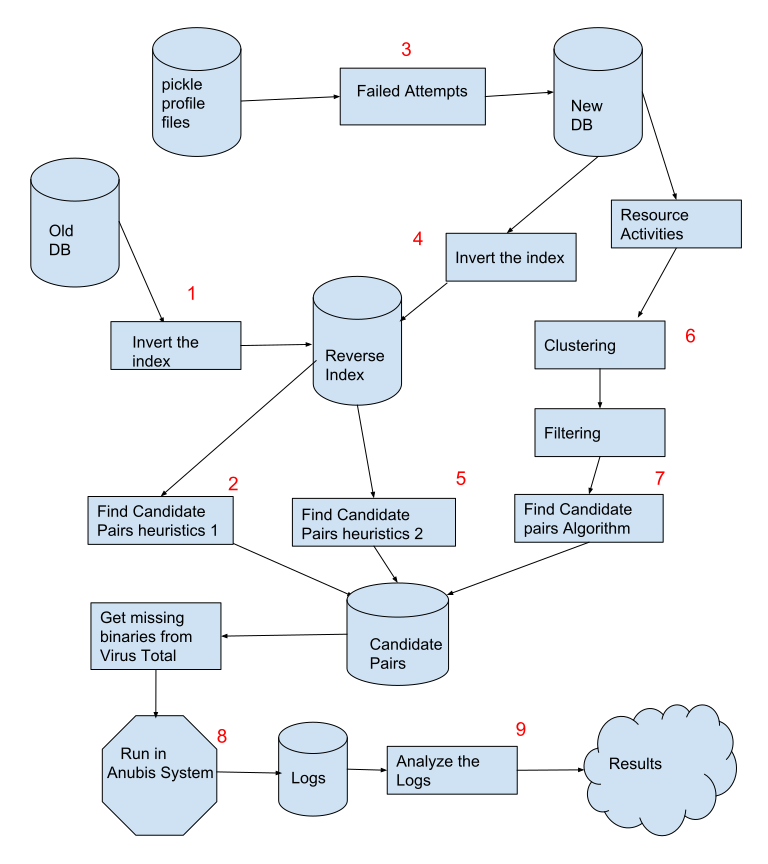
\includegraphics[scale=0.4]{figures/bigpicture.png}
  \caption[Big Picture]{Illustration of how we planned to perform the experiment}\label{fig:bigpicture}
\end{figure}
\section{Research Tools}
\label{sec:Research Tools}
\subsection{Anubis}
\label{sub:Anubis}
\subsection{Python}
\label{sub:Python}
\subsection{MySql}
\label{sub:MySql}
\section{Topic model: LDA}
\label{sec:Topic model: LDA}
We started to explore different clustering approach of malware samples based on their activities, into different Topics/families.
To cluster the malware we had multiple options. We looked into the behavioral-clustering paper by~\cite[Bayer]{bayer}.
The clustering results were for tens of thousands of malware samples and not millions, and the approach still does not look like scalable to (16M) millions of samples.
The approach has a linear bootstrapping phase of Locality-sensitive hashing \(LSH\), after which the $O(n^2)$ hierarchical clustering starts.
The whole premise of faster execution lies within careful tuning of multiple parameters and hash functions (to make the initial phase take care of most of the load), which had not been done by the authors for millions of samples (the biggest execution they had was for 75K samples).
This means that we would have needed to tune and change the code as we go forward to get the results we hope for.
Instead we preferred using something ready to use (not to spend time improving something that would not be considered any novelty for our work).
\\
Another alternative was VirusTotal labels (which we will be using as additional information), but unfortunately are not very accurate.
\\
A third approach was to use a clustering algorithm that is scalable, but maybe less accurate than the behavioral clustering, but able to cluster millions of samples.
We decided to map the problem to document clustering (considering each malware as a document, and the its resource activities as its words).
As {tf-idf} approaches have a large memory footprint $(O(\#docs \times \#words))$, we switched to clustering algorithms whose memory footprint does not depend on the number of documents.
\\
Latent Dirichlet allocation\(LDA\), equivalent to dimension-reduction algorithms for high-dimensional clustering, is one such algorithm and its memory footprint is $(O(\#docs \times \#words))$. This gives us a more fine grained clustering compared to previously proposed LHS (Locality-sensitive hashing) based approach.
\section{Running Experiment}
\label{sec:Running Experiment}
\begin{itemize}
  \item Say, \emph{R} is a set of candidate resources such that each resource ``r'' in \emph{R} have some malware set that create it (say set $A_r$) and some other set of malware that try to (unsuccessfully) access/delete it (say set $B_r$).
    \item We combine all such sets $A_r$ and $B_r$ corresponding to ``r'' in \emph{R} to sets \emph{A} and \emph{B}, respectively. Combine `A' and `B' and cluster them to cluster ids $[c_1,c_2,\ldots.\ c_n]$ (\emph{n} is family/topic count) such that any malware sample \emph{x} in (\emph{A} union \emph{B}) can be tagged/mapped to cluster id $C(x)$, where $C(x)$ belongs to $[c_1, c_2, \ldots c_n]$.
    \item Now, for each ``r'' in \emph{R}, we generate a set of candidate pairs $p_r$ for experiment. $p_r$ is a set of malware pairs $(x_r, y_r)$ such that $x_r$ belongs to $A_r$ and $y_r$ belongs to $B_r$ and $C(x_r)$ not equal to $C(y_r)$, not belonging to same cluster.
    \item We generate such $(x_r, y_r)$ pairs for all possible cluster pairs $(C(x_r), C(y_r))$ corresponding to a resource ``r''.
    \item The final experiment set \emph{E} is a set of such $(x_r, y_r)$ for all resources \emph{r} in \emph{R}.
    \item Finally for any resource ``r'', if the size of the set $| C(x) : x \in A_r | > 10 or  | C(x) : x \in B_r | > 10$, we discard \emph{r} and its corresponding experiment pairs from \emph{E}, since the resource created/read by too many families is less interesting.
    \item Here $(x,y)$ and $(y,x)$ will be different experiments because we run one sample, wait, and run another sample. Result can be different based on which one runs first. In rare case, both samples may be trying detect each other.

\end{itemize}




Citation test~\parencite{latex}.
